\documentclass[a4paper,12pt]{report}

\usepackage{cmap}
\usepackage[T2A]{fontenc}
\usepackage[utf8]{inputenc}
\usepackage[english,russian]{babel}
\usepackage{listings}
\usepackage{amsmath}
\usepackage{amsfonts}
\usepackage{float}
\usepackage{csquotes}
\usepackage{hyphenat}

% \usepackage{titlesec}
% \newcommand{\sectionbreak}{\clearpage}

\usepackage{graphicx}
\graphicspath{ {./images/} }

\usepackage{xcolor}
% \usepackage{courier}

\usepackage[
    backend=biber,
    style=alphabetic,
    sorting=ynt
]{biblatex}
\addbibresource{resources.bib}

\definecolor{buzzlightyear}{HTML}{8757A5}
\definecolor{grass}{HTML}{738D06}
\definecolor{sand}{HTML}{F18A2B}
\definecolor{comment}{HTML}{8E908B}

\lstdefinestyle{habrstyle}{
    backgroundcolor=\color{white},   
    commentstyle=\color{comment},
    keywordstyle=\bfseries\color{buzzlightyear},
    numberstyle=\tiny\color{comment},
    stringstyle=\color{grass},
    basicstyle=\ttfamily\footnotesize,
    breakatwhitespace=false,         
    breaklines=true,                 
    captionpos=b,                    
    keepspaces=true,                 
    numbers=left,                    
    numbersep=5pt,                  
    showspaces=false,                
    showstringspaces=false,
    showtabs=false,                  
    tabsize=4
}

\lstset{style=habrstyle}

\author{Луняк Николай}
\title{Лабораторная работа 9}
\date{\today}

\begin{document}
    \maketitle
    \tableofcontents
    \listoffigures
    \lstlistoflistings
    
    \chapter{Багаж импортов}
    
    Разные штуки, которые часто оказываются необходимыми.
    
\begin{lstlisting}[language=Python,caption=Импорты]
from thinkdsp import Signal, Sinusoid, SquareSignal, TriangleSignal, SawtoothSignal, ParabolicSignal
from thinkdsp import normalize, unbias, PI2, decorate
from thinkdsp import Chirp
from thinkdsp import read_wave
from thinkdsp import Spectrum, Wave, UncorrelatedGaussianNoise, Spectrogram
from thinkdsp import Noise

import numpy as np
import pandas as pd

from matplotlib import pyplot as plt

import thinkstats2

from scipy.stats import linregress

import scipy
import scipy.fftpack

import scipy.signal

from ipywidgets import interact, interactive, fixed
import ipywidgets as widgets

loglog = dict(xscale='log', yscale='log')

PI2 = np.pi * 2
\end{lstlisting}

    \chapter{Сравнение \texttt{diff} и \texttt{differentiate} на примере треугольного сигнала}

    Создадим треугольный сигнал:
    
\begin{lstlisting}[language=Python,caption=Создаем треугольный сигнал]
in_wave = TriangleSignal(freq=50).make_wave(duration=0.1, framerate=44100)
in_wave.plot()
decorate(xlabel='Time (s)')
\end{lstlisting}

    \begin{figure}[H]
        \centering
        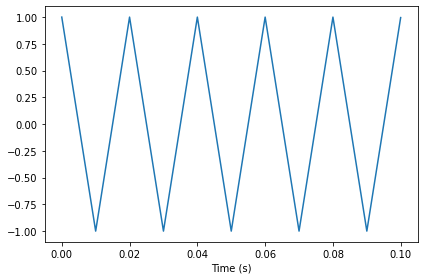
\includegraphics[width=0.75\textwidth]{ex1_in_wave.png}
        \caption{Исходный сигнал}
        \label{fig:ex1_in_wave}
    \end{figure}

    Посчитаем его производную численно:
    
\begin{lstlisting}[language=Python,caption=Делаем \texttt{diff}]
out_wave = in_wave.diff()
out_wave.plot()
decorate(xlabel='Time (s)')
\end{lstlisting}

    \begin{figure}[H]
        \centering
        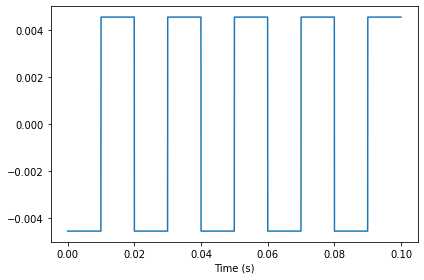
\includegraphics[width=0.75\textwidth]{ex1_out_wave.png}
        \caption{После \texttt{diff}}
        \label{fig:ex1_out_wave}
    \end{figure}

    Получился прямоугольный сигнал. Теперь возьмем спектр:
    
\begin{lstlisting}[language=Python,caption=Спектр]
in_spectrum = in_wave.make_spectrum()
in_spectrum.plot(high=2000)
decorate(xlabel='Frequency (1/s)')
\end{lstlisting}

    \begin{figure}[H]
        \centering
        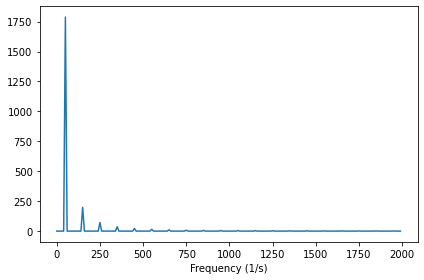
\includegraphics[width=0.75\textwidth]{ex1_in_spectrum.png}
        \caption{Спектр}
        \label{fig:ex1_in_spectrum}
    \end{figure}

    Получим его производную:
    
\begin{lstlisting}[language=Python,caption=Продифференциированный спектр]
out_spectrum = in_spectrum.differentiate()
out_spectrum.plot(high=2000)
decorate(xlabel='Frequency (1/s)')
\end{lstlisting}

    \begin{figure}[H]
        \centering
        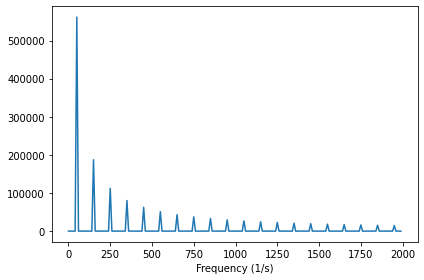
\includegraphics[width=0.75\textwidth]{ex1_out_spectrum.png}
        \caption{Продифференциированный спектр}
        \label{fig:ex1_out_spectrum}
    \end{figure}

    А теперь превратим обратно в сигнал во времени;
    
\begin{lstlisting}[language=Python,caption=Новый сигнал]
out_wave2 = out_spectrum.make_wave()
out_wave2.plot()
decorate(xlabel='Time (s)')
\end{lstlisting}

    \begin{figure}[H]
        \centering
        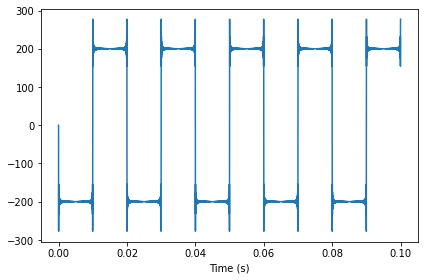
\includegraphics[width=0.75\textwidth]{ex1_out_wave2.png}
        \caption{Новый сигнал}
        \label{fig:ex1_out_wave2}
    \end{figure}

    И мы снова получили прямоугольный сигнал, правда в этот раз заметно более \textquote{плохого качества} (края плохо аппроксимируются конечным числом синусоид).
    
    \chapter{Сравнение \texttt{cumsum} и \texttt{integrate} на примере прямоугольного сигнала}
    
    Уже по названию напрашивается аналогия с прошлым разделом, но убедимся в этмо более формально.
    
\begin{lstlisting}[language=Python,caption=Прямоугольный сигнал]
in_wave = SquareSignal(freq=50).make_wave(duration=0.1, framerate=44100)
in_wave.plot()
decorate(xlabel='Time (s)')
\end{lstlisting}

    \begin{figure}[H]
        \centering
        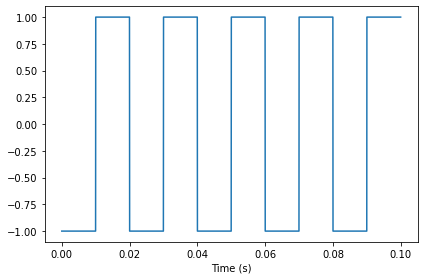
\includegraphics[width=0.75\textwidth]{ex2_in_wave.png}
        \caption{Прямоугольный сигнал}
        \label{fig:ex2_in_wave}
    \end{figure}

    Считаем \texttt{cumsum}:
    
\begin{lstlisting}[language=Python,caption=\textquote{Просуммированный}]
out_wave = in_wave.cumsum()
out_wave.plot()
decorate(xlabel='Time (s)')
\end{lstlisting}

    \begin{figure}[H]
        \centering
        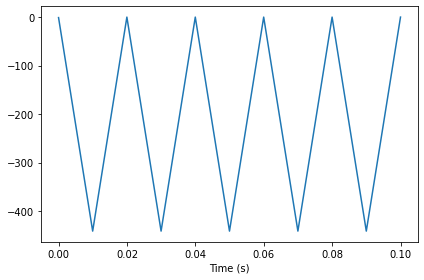
\includegraphics[width=0.75\textwidth]{ex2_out_wave.png}
        \caption{\textquote{Просуммированный}}
        \label{fig:ex2_out_wave}
    \end{figure}

    Теперь возьмем спектр:
    
\begin{lstlisting}[language=Python,caption=Спектр]
in_spectrum = in_wave.make_spectrum()
in_spectrum.hs[0] = 0
in_spectrum.plot(high=5000)
decorate(xlabel='Frequency (1/s)')
\end{lstlisting}

    \begin{figure}[H]
        \centering
        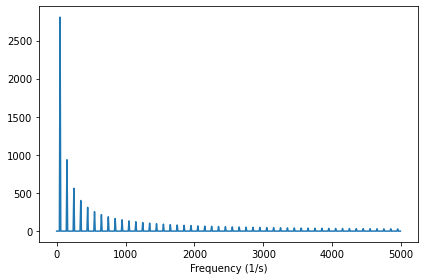
\includegraphics[width=0.75\textwidth]{ex2_in_spectrum.png}
        \caption{Спектр}
        \label{fig:ex2_in_spectrum}
    \end{figure}

    Интегрируем:
    
\begin{lstlisting}[language=Python,caption=Проинтегрированный сигнал]
out_spectrum = in_spectrum.integrate()
out_spectrum.hs[0] = 0
out_spectrum.plot(high=2000)
decorate(xlabel='Frequency (1/s)')
\end{lstlisting}

    \begin{figure}[H]
        \centering
        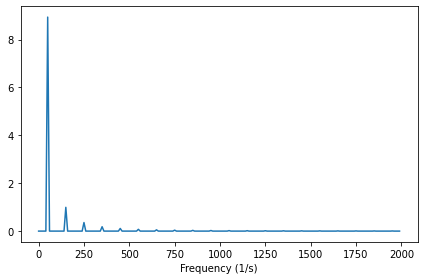
\includegraphics[width=0.75\textwidth]{ex2_out_spectrum.png}
        \caption{Проинтегрированный сигнал}
        \label{fig:ex2_out_spectrum}
    \end{figure}

    И превращаем в сигнал:
    
\begin{lstlisting}[language=Python,caption=Новый сигнал]
out_wave2 = out_spectrum.make_wave()
out_wave2.plot()
decorate(xlabel='Time (s)')
\end{lstlisting}

    \begin{figure}[H]
        \centering
        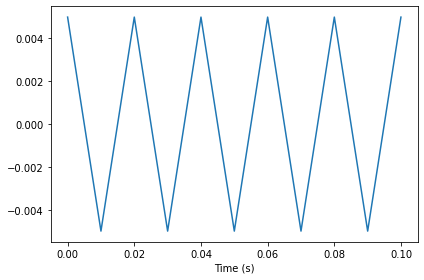
\includegraphics[width=0.75\textwidth]{ex2_out_wave2.png}
        \caption{Новый сигнал}
        \label{fig:ex2_out_wave2}
    \end{figure}

    А вот тут уже сигналы кажутся полностью одинаковыми, хотя и с точностью до линейной трансформации.
    
    \chapter{Двойное интегрирование на примере пилообразного сигнала}
    
\begin{lstlisting}[language=Python,caption=Пилообразный сигнал]
in_wave = SawtoothSignal(freq=50).make_wave(duration=0.1, framerate=44100)
in_wave.plot()
decorate(xlabel='Time (s)')
\end{lstlisting}

    \begin{figure}[H]
        \centering
        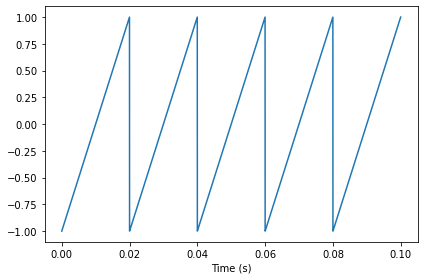
\includegraphics[width=0.75\textwidth]{ex3_in_wave.png}
        \caption{Пилообразный сигнал}
        \label{fig:ex3_in_wave}
    \end{figure}

    Считаем \texttt{cumsum}:
    
\begin{lstlisting}[language=Python,caption=\textquote{Просуммированный}]
out_wave = in_wave.cumsum()
out_wave.unbias()
out_wave.plot()
decorate(xlabel='Time (s)')
\end{lstlisting}

    \begin{figure}[H]
        \centering
        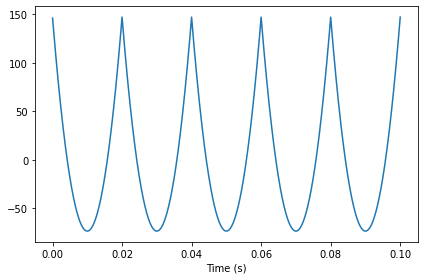
\includegraphics[width=0.75\textwidth]{ex3_out_wave.png}
        \caption{\textquote{Просуммированный}}
        \label{fig:ex3_out_wave}
    \end{figure}

    Еще считаем \texttt{cumsum}:
    
\begin{lstlisting}[language=Python,caption=\textquote{Просуммированный х2}]
out_wave = out_wave.cumsum()
out_wave.plot()
decorate(xlabel='Time (s)')
\end{lstlisting}

    \begin{figure}[H]
        \centering
        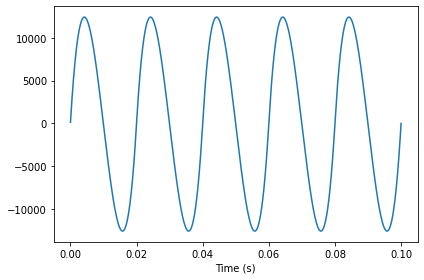
\includegraphics[width=0.75\textwidth]{ex3_in_wave_more.png}
        \caption{\textquote{Просуммированный х2}}
        \label{fig:ex3_in_wave_more}
    \end{figure}

    Теперь возьмем спектр:
    
\begin{lstlisting}[language=Python,caption=Спектр]
in_spectrum = in_wave.make_spectrum()
in_spectrum.hs[0] = 0
in_spectrum.plot(high=5000)
decorate(xlabel='Frequency (1/s)')
\end{lstlisting}

    \begin{figure}[H]
        \centering
        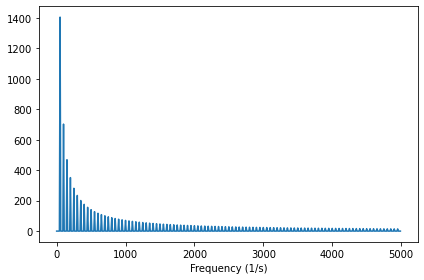
\includegraphics[width=0.75\textwidth]{ex3_in_spectrum.png}
        \caption{Спектр}
        \label{fig:ex3_in_spectrum}
    \end{figure}

    Интегрируем:
    
\begin{lstlisting}[language=Python,caption=Проинтегрированный спектр]
out_spectrum = in_spectrum.integrate()
out_spectrum.hs[0] = 0
out_spectrum.plot(high=2000)
decorate(xlabel='Frequency (1/s)')
\end{lstlisting}

    \begin{figure}[H]
        \centering
        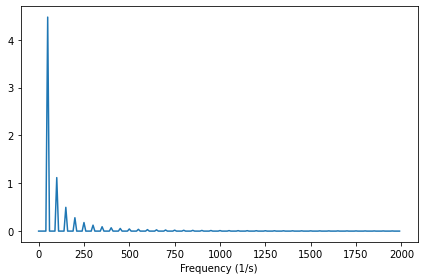
\includegraphics[width=0.75\textwidth]{ex3_out_spectrum.png}
        \caption{Проинтегрированный спектр}
        \label{fig:ex3_out_spectrum}
    \end{figure}

    Снова интегрируем:
    
\begin{lstlisting}[language=Python,caption=Проинтегрированный спектр х2]
out_spectrum = out_spectrum.integrate()
out_spectrum.hs[0] = 0
out_spectrum.plot(high=500)
decorate(xlabel='Frequency (1/s)')
\end{lstlisting}

    \begin{figure}[H]
        \centering
        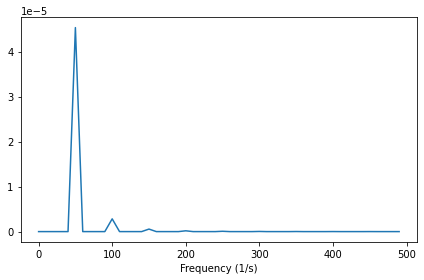
\includegraphics[width=0.75\textwidth]{ex3_out_spectrum_more.png}
        \caption{Проинтегрированный спектр х2}
        \label{fig:ex3_out_spectrum_more}
    \end{figure}

    И превращаем в сигнал:
    
\begin{lstlisting}[language=Python,caption=Новый сигнал]
out_wave2 = out_spectrum.make_wave()
out_wave2.plot()
decorate(xlabel='Time (s)')
\end{lstlisting}

    \begin{figure}[H]
        \centering
        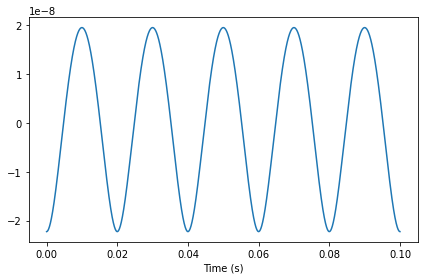
\includegraphics[width=0.75\textwidth]{ex3_out_wave2.png}
        \caption{Новый сигнал}
        \label{fig:ex3_out_wave2}
    \end{figure}

    Тут \textquote{вторая версия} более похожа на синусоиду, чем первая. Можно вот так вот сравнить еще:
    
\begin{lstlisting}[language=Python,caption=Сравнение]
out_wave.normalize()
out_wave.unbias()
out_wave.plot()

out_wave2.normalize()
out_wave2.unbias()
out_wave2.plot()

decorate(xlabel='Time (s)')
\end{lstlisting}

    \begin{figure}[H]
        \centering
        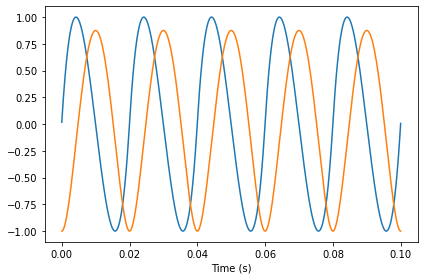
\includegraphics[width=0.75\textwidth]{ex3_comparison.png}
        \caption{Сравнение}
        \label{fig:ex3_comparison}
    \end{figure}

    Можно видеть, что первая чуть сильнее наклоняется влево. Впрочем, ни то, ни то не есть синусоида, просто большие частоты подавляются, но не полностью идеально, поэтому нам может казаться, что это синусоиды.
    
    \chapter{Двойное дифференциирование на примере кубического сигнала}
    
\begin{lstlisting}[language=Python,caption=Кубический сигнал]
from thinkdsp import CubicSignal
in_wave = CubicSignal(freq=0.0005).make_wave(duration=10000, framerate=1)
in_wave.plot()
\end{lstlisting}

    \begin{figure}[H]
        \centering
        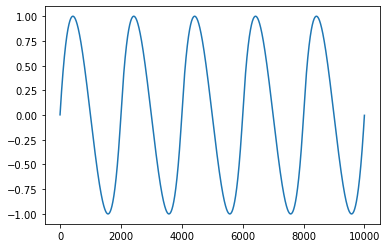
\includegraphics[width=0.75\textwidth]{ex4_in_wave.png}
        \caption{Кубический сигнал}
        \label{fig:ex4_in_wave}
    \end{figure}

    Перед тем, как продолжить, хотелось бы сразу посмотреть на спектр:
    
\begin{lstlisting}[language=Python,caption=Спектр]
in_wave.make_spectrum().plot(high=0.006)
\end{lstlisting}

    \begin{figure}[H]
        \centering
        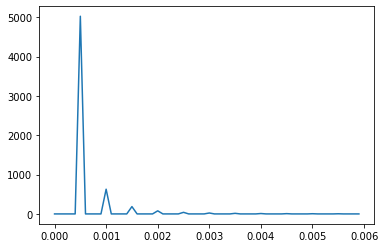
\includegraphics[width=0.75\textwidth]{ex4_in_wave_spectrum.png}
        \caption{Спектр}
        \label{fig:ex4_in_wave_spectrum}
    \end{figure}

    Ага, это уже больше похоже на результаты прошлого раздела. У нас есть некоторая значимая низкая частота, и \textquote{что-то там еще} после нее, и в итоге сигнал кажется наклоненным. Впрочем, вот так вот \textquote{на глаз} нельзя говорить, что мы получили в прошлом разделе именно кубический сигнал, кривизну нужно доказывать.

    Посчитаем \texttt{diff}:
    
\begin{lstlisting}[language=Python,caption=Применили \texttt{diff}]
out_wave = in_wave.diff()
out_wave.plot()
\end{lstlisting}

    \begin{figure}[H]
        \centering
        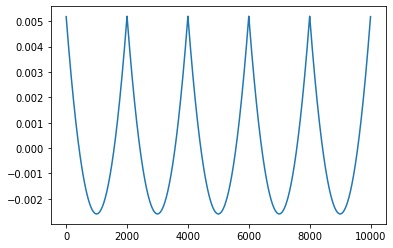
\includegraphics[width=0.75\textwidth]{ex4_out_wave.png}
        \caption{Применили \texttt{diff}}
        \label{fig:ex4_out_wave}
    \end{figure}

    Еще считаем \texttt{diff}:
    
\begin{lstlisting}[language=Python,caption=Применили \texttt{diff} х2]
out_wave = out_wave.diff()
out_wave.plot()
\end{lstlisting}

    \begin{figure}[H]
        \centering
        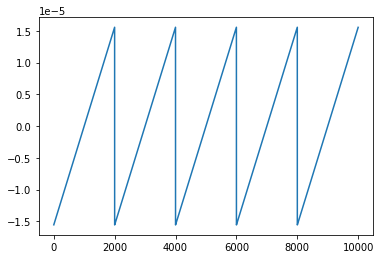
\includegraphics[width=0.75\textwidth]{ex4_out_wave_more.png}
        \caption{Применили \texttt{diff} х2}
        \label{fig:ex4_out_wave_more}
    \end{figure}

    Теперь возьмем спектр:
    
\begin{lstlisting}[language=Python,caption=Спектр]
in_spectrum = in_wave.make_spectrum()
in_spectrum.plot(high=0.01)
decorate(xlabel='Frequency (1/s)')
\end{lstlisting}

    \begin{figure}[H]
        \centering
        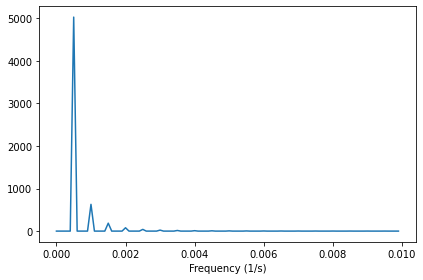
\includegraphics[width=0.75\textwidth]{ex4_in_spectrum.png}
        \caption{Спектр}
        \label{fig:ex4_in_spectrum}
    \end{figure}

    Дифференциируем:
    
\begin{lstlisting}[language=Python,caption=Продифференциированный спектр]
out_spectrum = in_spectrum.differentiate()
out_spectrum.plot(high=0.01)
decorate(xlabel='Frequency (1/s)')
\end{lstlisting}

    \begin{figure}[H]
        \centering
        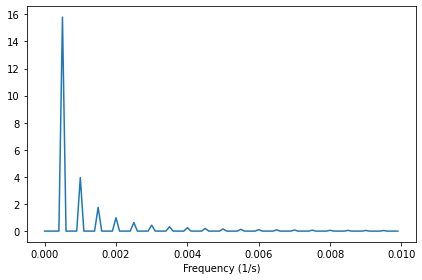
\includegraphics[width=0.75\textwidth]{ex4_out_spectrum.png}
        \caption{Продифференциированный спектр}
        \label{fig:ex4_out_spectrum}
    \end{figure}

    Снова дифференциируем:
    
\begin{lstlisting}[language=Python,caption=Продифференциированный спектр х2]
out_spectrum = out_spectrum.differentiate()
out_spectrum.plot(high=0.04)
decorate(xlabel='Frequency (1/s)')
\end{lstlisting}
    
    \begin{figure}[H]
        \centering
        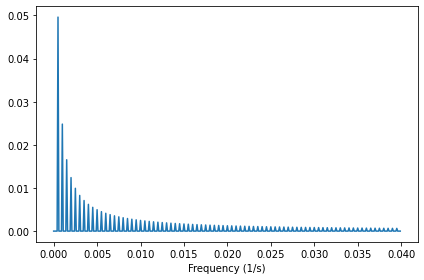
\includegraphics[width=0.75\textwidth]{ex4_out_spectrum_more.png}
        \caption{Продифференциированный спектр х2}
        \label{fig:ex4_out_spectrum_more}
    \end{figure}

    И превращаем в сигнал:
    
\begin{lstlisting}[language=Python,caption=Новый сигнал]
out_wave2 = out_spectrum.make_wave()
out_wave2.plot()
decorate(xlabel='Time (s)')
\end{lstlisting}

    \begin{figure}[H]
        \centering
        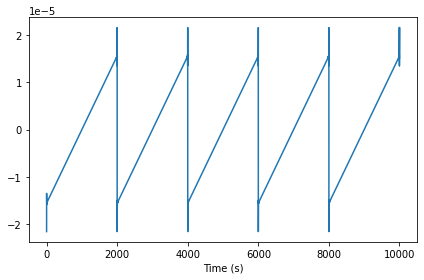
\includegraphics[width=0.75\textwidth]{ex4_out_wave2.png}
        \caption{Новый сигнал}
        \label{fig:ex4_out_wave2}
    \end{figure}

    Да, пожалуй, это тоже пилообразный сигнал, хотя мы наблюдаем эффект, аналогичный первому разделу с неточной аппроксимацией.
    
    Рассмотрим соответствующие фильтры. Из Вычислительной математики знаем окно, соответствующее второй численной производной, так что просто берем ее DFT.
    
\begin{lstlisting}[language=Python,caption=Фильтр для \texttt{difference} x2]
from thinkdsp import zero_pad

diff_window = np.array([-1.0, 2.0, -1.0])
padded = zero_pad(diff_window, len(in_wave))
diff_wave = Wave(padded, framerate=in_wave.framerate)

diff_filter = diff_wave.make_spectrum()
diff_filter.plot(label='2nd diff')
decorate(xlabel='Frequency (Hz)', ylabel='Amplitude ratio')
\end{lstlisting}

    \begin{figure}[H]
        \centering
        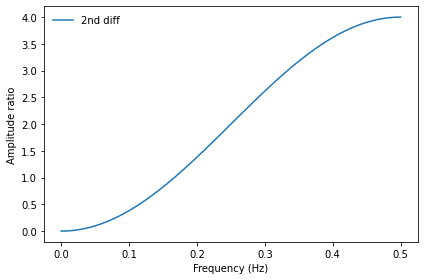
\includegraphics[width=0.75\textwidth]{ex4_window_1.png}
        \caption{Фильтр для \texttt{difference} x2}
        \label{fig:ex4_window_1}
    \end{figure}

    Фильтр для второй производной есть квадрат фильтра первой.
    
\begin{lstlisting}[language=Python,caption=Фильтр для \texttt{differentiate} x2]
deriv_filter = in_wave.make_spectrum()
deriv_filter.hs = (PI2 * 1j * deriv_filter.fs)**2
deriv_filter.plot(label='2nd deriv')
decorate(xlabel='Frequency (Hz)', ylabel='Amplitude ratio')
\end{lstlisting}

    \begin{figure}[H]
        \centering
        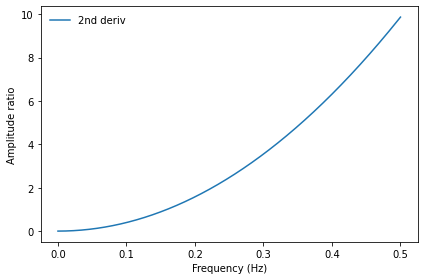
\includegraphics[width=0.75\textwidth]{ex4_window_2.png}
        \caption{Фильтр для \texttt{differentiate} x2}
        \label{fig:ex4_window_2}
    \end{figure}

    Удобно смотреть вместе на оба фильтра.
    
\begin{lstlisting}[language=Python,caption=Сравнение]
diff_filter.plot(label='2nd diff')
deriv_filter.plot(label='2nd deriv')
decorate(xlabel='Frequency (Hz)', ylabel='Amplitude ratio')
\end{lstlisting}

    \begin{figure}[H]
        \centering
        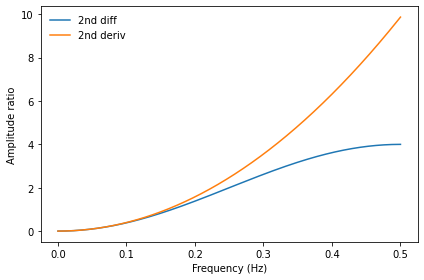
\includegraphics[width=0.75\textwidth]{ex4_window_comparison.png}
        \caption{Сравнение}
        \label{fig:ex4_window_comparison}
    \end{figure}

    Поначалу они очень похожи, но вот для больших частот начинают сильно расходиться.

    % \printbibliography
    
\end{document}
